\documentclass{beamer}\usepackage[]{graphicx}\usepackage[]{color}
%% maxwidth is the original width if it is less than linewidth
%% otherwise use linewidth (to make sure the graphics do not exceed the margin)
\makeatletter
\def\maxwidth{ %
  \ifdim\Gin@nat@width>\linewidth
    \linewidth
  \else
    \Gin@nat@width
  \fi
}
\makeatother

\definecolor{fgcolor}{rgb}{0.345, 0.345, 0.345}
\newcommand{\hlnum}[1]{\textcolor[rgb]{0.686,0.059,0.569}{#1}}%
\newcommand{\hlstr}[1]{\textcolor[rgb]{0.192,0.494,0.8}{#1}}%
\newcommand{\hlcom}[1]{\textcolor[rgb]{0.678,0.584,0.686}{\textit{#1}}}%
\newcommand{\hlopt}[1]{\textcolor[rgb]{0,0,0}{#1}}%
\newcommand{\hlstd}[1]{\textcolor[rgb]{0.345,0.345,0.345}{#1}}%
\newcommand{\hlkwa}[1]{\textcolor[rgb]{0.161,0.373,0.58}{\textbf{#1}}}%
\newcommand{\hlkwb}[1]{\textcolor[rgb]{0.69,0.353,0.396}{#1}}%
\newcommand{\hlkwc}[1]{\textcolor[rgb]{0.333,0.667,0.333}{#1}}%
\newcommand{\hlkwd}[1]{\textcolor[rgb]{0.737,0.353,0.396}{\textbf{#1}}}%
\let\hlipl\hlkwb

\usepackage{framed}
\makeatletter
\newenvironment{kframe}{%
 \def\at@end@of@kframe{}%
 \ifinner\ifhmode%
  \def\at@end@of@kframe{\end{minipage}}%
  \begin{minipage}{\columnwidth}%
 \fi\fi%
 \def\FrameCommand##1{\hskip\@totalleftmargin \hskip-\fboxsep
 \colorbox{shadecolor}{##1}\hskip-\fboxsep
     % There is no \\@totalrightmargin, so:
     \hskip-\linewidth \hskip-\@totalleftmargin \hskip\columnwidth}%
 \MakeFramed {\advance\hsize-\width
   \@totalleftmargin\z@ \linewidth\hsize
   \@setminipage}}%
 {\par\unskip\endMakeFramed%
 \at@end@of@kframe}
\makeatother

\definecolor{shadecolor}{rgb}{.97, .97, .97}
\definecolor{messagecolor}{rgb}{0, 0, 0}
\definecolor{warningcolor}{rgb}{1, 0, 1}
\definecolor{errorcolor}{rgb}{1, 0, 0}
\newenvironment{knitrout}{}{} % an empty environment to be redefined in TeX

\usepackage{alltt}

\usepackage{default}
\usepackage{animate} %need the animate.sty file 
\usepackage{graphicx}
%\graphicspath{{/home/sahir/Dropbox/jobs/laval/minicours/slides/}}
\usepackage{hyperref, url}
%\usepackage[round,sort]{natbib}   % bibliography omit 'round' option if you prefer square brackets
%\bibliographystyle{apalike}
\usepackage{biblatex}
\bibliography{bib.bib}
% Removes icon in bibliography
\setbeamertemplate{bibliography item}[text]

\usepackage[normalem]{ulem}

\setbeamertemplate{theorems}[numbered]



%\newtheorem{prop}{Proposition}
%\newenvironment{theoremc}[1]
%{\begin{shaded}\begin{theorem}[#1]}
%		{\end{theorem}\end{shaded}}
	
%\newtheorem{examplefirst}{Example}
%\newtheorem{examplesecond}{Example}
%\newenvironment<>{examplefirst}[1][]{%
%	\setbeamercolor{block title example}{bg=lightgray}%
%	\begin{example}#2[#1]}{\end{example}}
%\newenvironment<>{examplesecond}[1][]{%
%	\setbeamercolor{block title example}{fg=white,bg=blue!75!black}%
%	\begin{example}#2[#1]}{\end{example}}	

%\usepackage{amsthm}


\usepackage[figurename=Fig.]{caption}
\usepackage{subfig}
\usepackage{tikz, pgfplots,epsfig}
\usetikzlibrary{arrows,shapes.geometric}
\usepackage{color, colortbl,xcolor}
\definecolor{lightgray}{RGB}{200,200,200}
\definecolor{palegray}{RGB}{221,221,221}
\definecolor{myblue}{RGB}{0,89,179}
\usepackage{comment}
\setbeamercolor{frametitle}{fg=myblue}
\setbeamercolor{section in head/foot}{bg=myblue, fg=white}
\setbeamercolor{author in head/foot}{bg=myblue}
\setbeamercolor{date in head/foot}{bg=myblue}

\usepackage{shadethm}
%\colorlet{shadecolor}{blue!15}
\colorlet{shadecolor}{palegray}
%\setlength{\shadeboxrule}{.4pt}

\newshadetheorem{thm}{Theorem}
\newshadetheorem{defm}{Definition}
\newshadetheorem{exm}{Exercise}
\newshadetheorem{remarkm}{Remark}
%\definecolor{shadethmcolor}{HTML}{EDF8FF}
\definecolor{shadethmcolor}{RGB}{221,221,221}
%\definecolor{shaderulecolor}{HTML}{45CFFF}
\definecolor{shaderulecolor}{RGB}{0,89,179}
\setlength{\shadeboxrule}{.4pt}


\usepackage{array}
\newcolumntype{L}{>{\centering\arraybackslash}m{3cm}} % used for text wrapping in ctable
\usepackage{ctable}
\usepackage[utf8]{inputenc}
\usepackage{fontenc}
\usepackage{pifont}% http://ctan.org/pkg/pifont
\newcommand{\cmark}{\ding{51}}%
\newcommand{\xmark}{\ding{55}}%
\def\widebar#1{\overline{#1}}
\definecolor{whitesmoke}{rgb}{0.96, 0.96, 0.96}

\usepackage{amssymb}
\usepackage{amsmath}

\usepackage{bm}
\def\transpose{{\sf{T}}}
\def\E{{\skew0\bm{E}}}
\def\Xvec{{\skew0\bm{X}}}
\def\Xveca{{\skew0\bm{X}}_1}
\def\Xvecb{{\skew0\bm{X}}_2}

\def\Yvec{{\skew0\bm{Y}}}
\def\bmY{{\skew0\bm{Y}}}
\def\bmX{{\skew0\bm{X}}}
\def\bmy{{\skew0\bm{y}}}
\def\bmG{{\skew0\bm{G}}}
\def\bmS{{\skew0\bm{S}}}
\def\bmA{{\skew0\bm{A}}}
\def\bmB{{\skew0\bm{B}}}
\def\bmD{{\skew0\bm{D}}}
\def\bmI{{\skew0\bm{I}}}
\def\bmV{{\skew0\bm{V}}}
\def\bmU{{\skew0\bm{U}}}
\def\bv{{\skew0\bm{v}}}
\def\bw{{\skew0\bm{w}}}
\def\bmm{{\skew0\bm{m}}}
\def\bmzero{{\skew0\bm{0}}}
\def\bx{{\skew0\bm{x}}}
\def\xveca{{\skew0\bm{x}}_1}
\def\xvecb{{\skew0\bm{x}}_2}

\def\N{{\skew0\mathcal{N}}}
\def\T{{\small T}}

\def\mvec{{\skew0\bm{m}}}
\def\bmmu{{\skew0\bm{\mu}}}
\def\muvec{{\skew0\bm{\mu}}}
\def\balpha{{\skew0\bm{\alpha}}}
\def\bbeta{{\skew0\bm{\beta}}}
\def\bmtheta{{\skew0\bm{\theta}}}
\def\btheta{{\skew0\bm{\theta}}}

\def\cvec{{\skew0\mathbf{c}}}

\def\Xbar{\overline{X}}

\definecolor{lightgray}{rgb}{0.91,0.91,0.91}
\definecolor{purpleblue}{rgb}{0.50,0.50,1.00}



\usepackage{fontspec}
%\setsansfont{Fira Sans}
%\setmonofont{Fira Mono}
\setsansfont[ItalicFont={Fira Sans Light Italic},BoldFont={Fira Sans},BoldItalicFont={Fira Sans Italic}]{Fira Sans Light}
\setmonofont[BoldFont={Fira Mono Medium}]{Fira Mono}


\setbeamercolor{itemize item}{fg=myblue}
\setbeamertemplate{itemize item}[square]

\setbeamertemplate{navigation symbols}{\usebeamercolor[fg]{title in head/foot}\usebeamerfont{title in head/foot}\insertframenumber}
\setbeamertemplate{footline}{}

\newtheorem{proposition}[theorem]{Proposition}
\newtheorem{exercise}[theorem]{Exercise}

\titlegraphic{\hfill
\includegraphics[height=1cm]{mcgill_logo.png}}


%% You also use hyperref, and pick colors 
\hypersetup{colorlinks,citecolor=orange,filecolor=red,linkcolor=brown,urlcolor=blue}

\newcommand {\framedgraphiccaption}[2] {
	\begin{figure}
		\centering
		\includegraphics[width=\textwidth,height=0.8\textheight,keepaspectratio]{#1}
		\caption{#2}
	\end{figure}
}

\newcommand {\framedgraphic}[1] {
	\begin{figure}
		\centering
		\includegraphics[width=\textwidth,height=0.9\textheight,keepaspectratio]{#1}
	\end{figure}
}


\AtBeginSection[]{
	\begin{frame}
		\vfill
		\centering
		\begin{beamercolorbox}[sep=8pt,center,shadow=true,rounded=true]{title}
			\usebeamerfont{title}\insertsectionhead\par%
		\end{beamercolorbox}
		\vfill
	\end{frame}
}

\newcommand\Wider[2][3em]{%
	\makebox[\linewidth][c]{%
		\begin{minipage}{\dimexpr\textwidth+#1\relax}
			\raggedright#2
		\end{minipage}%
	}%
}



\newcommand{\blue}[1]{\textcolor{blue}{#1}}
\newcommand{\red}[1]{\textcolor{red}{#1}}
%\makeatother

\usepackage{xparse}
\NewDocumentCommand\mylist{>{\SplitList{;}}m}
{
	\begin{itemize}
		\ProcessList{#1}{ \insertitem }
	\end{itemize}
}
\NewDocumentCommand\mynum{>{\SplitList{;}}m}
{
	\begin{enumerate}
		\ProcessList{#1}{ \insertitem }
	\end{enumerate}
}
\newcommand\insertitem[1]{\item #1}

\newcommand\FrameText[1]{%
	\begin{textblock*}{\paperwidth}(0pt,\textheight)
		\raggedright #1\hspace{.5em}
\end{textblock*}}
\IfFileExists{upquote.sty}{\usepackage{upquote}}{}
\begin{document}
%\sffamily



%\title{Introduction to Regression Trees}
%\author{Sahir Bhatnagar \inst{1}}
%\author[shortname]{Sahir Rai Bhatnagar, PhD Candidate (Biostatistics) }
%\institute[shortinst]{Department of Epidemiology, Biostatistics and Occupational Health}

\title{Inference about a Population Proportion ($\pi$)}
\subtitle{AAO unit 28; Baldi \& Moore, Ch 19}
\author{Sahir Bhatnagar and James Hanley}
\institute{
	EPIB 607\\
	Department of Epidemiology, Biostatistics, and Occupational Health\\
	McGill University\\
	
	\vspace{0.1 in}
	
	\texttt{sahir.bhatnagar@mcgill.ca}\\
	\texttt{\url{https://sahirbhatnagar.com/EPIB607/}}}

%\date

\maketitle

\section{Binomial Model for Sampling Variability of Proportion/Count in a Sample}




\begin{frame}
\frametitle{The Binomial Distribution: what it is}
\small
\begin{itemize}
	\setlength\itemsep{0.5em}
	\item It is the $n+1$ probabilities $p_{0}, p_{1}, ..., p_{y}, ..., p_{n}$ of observing 
	$0, 1, 2, \dots , n$ ``positives''  in \underline{$n$ independent realizations of a Bernoulli random variable} $Y$:
	$$
	Y = \begin{cases}
	1 & P(Y=1) = \pi \\
	0 & P(Y=0) = 1-\pi
	\end{cases}	
	$$
	The number is the sum of $n$ i.i.d. Bernoulli random variables.
	(\emph{such as in SRS of $n$ individuals}) \pause 
	\item Each of the $n$ observed elements is binary (0 or 1) \pause 
	\item There are $2^{n}$ possible \textit{sequences} ... but only $n+1$ possible \textit{values}, 
	i.e. $0/n,\;1/n,\;\dots ,\;n/n$  \emph{(can think of $y$ as sum of $n$ Bernoulli random variables)} 
	\item Note: it is better to work in same scale as the parameter, i.e., in [0,1]. Not the [0,n] count scale.
\end{itemize}
\end{frame}	
	
\begin{frame}
\frametitle{The Binomial Distribution: what it is}
\begin{itemize}
		\setlength\itemsep{0.5em}
	\item Apart from  ($n$), the probabilities $p_{0}$ to $p_{n}$ depend on only 1 parameter:
	\begin{itemize}
		\item the probability that a selected individual will be ``positive''  i.e.,
		\item the proportion of ``positive'' individuals in sampled population
	\end{itemize}

	\item Usually denote this (un-knowable) proportion by $\pi$
	
	\begin{tabular}{lcc}
		\hline
		Author & \textbf{Parameter} & \textbf{Statistic} \\
		\hline
		Clayton \& Hills   & $\pi $ & $p= D/N$ \\
		Hanley et al. & $\pi $ & $p= y/n$ \\
		M\&M, Baldi \& Moore & p &$\hat{p} = y/n$ \\
		Miettinen& P & $p=y/n$ \\
		\hline
	\end{tabular}
	\item
	Shorthand:  $Y\sim\; \textrm{Binomial}(n, \pi)$.
\end{itemize}
\end{frame}


\frame{\frametitle{Example} 
	
\begin{itemize}
	\setlength\itemsep{1em}
	\item Suppose a woman plans to have 3 children. 
	\item Suppose at each birth, 
	$$P(\textrm{female child}) = 1/2$$ and the sex of the child at each birth is
	independent of the sex at any previous birth. 
	\item What is the probability of having all daughters?
\end{itemize} 

}

\frame{\frametitle{The binomial distribution}
	
	\vspace*{-0.5in}
	
	\begin{figure}
		\begin{center}
			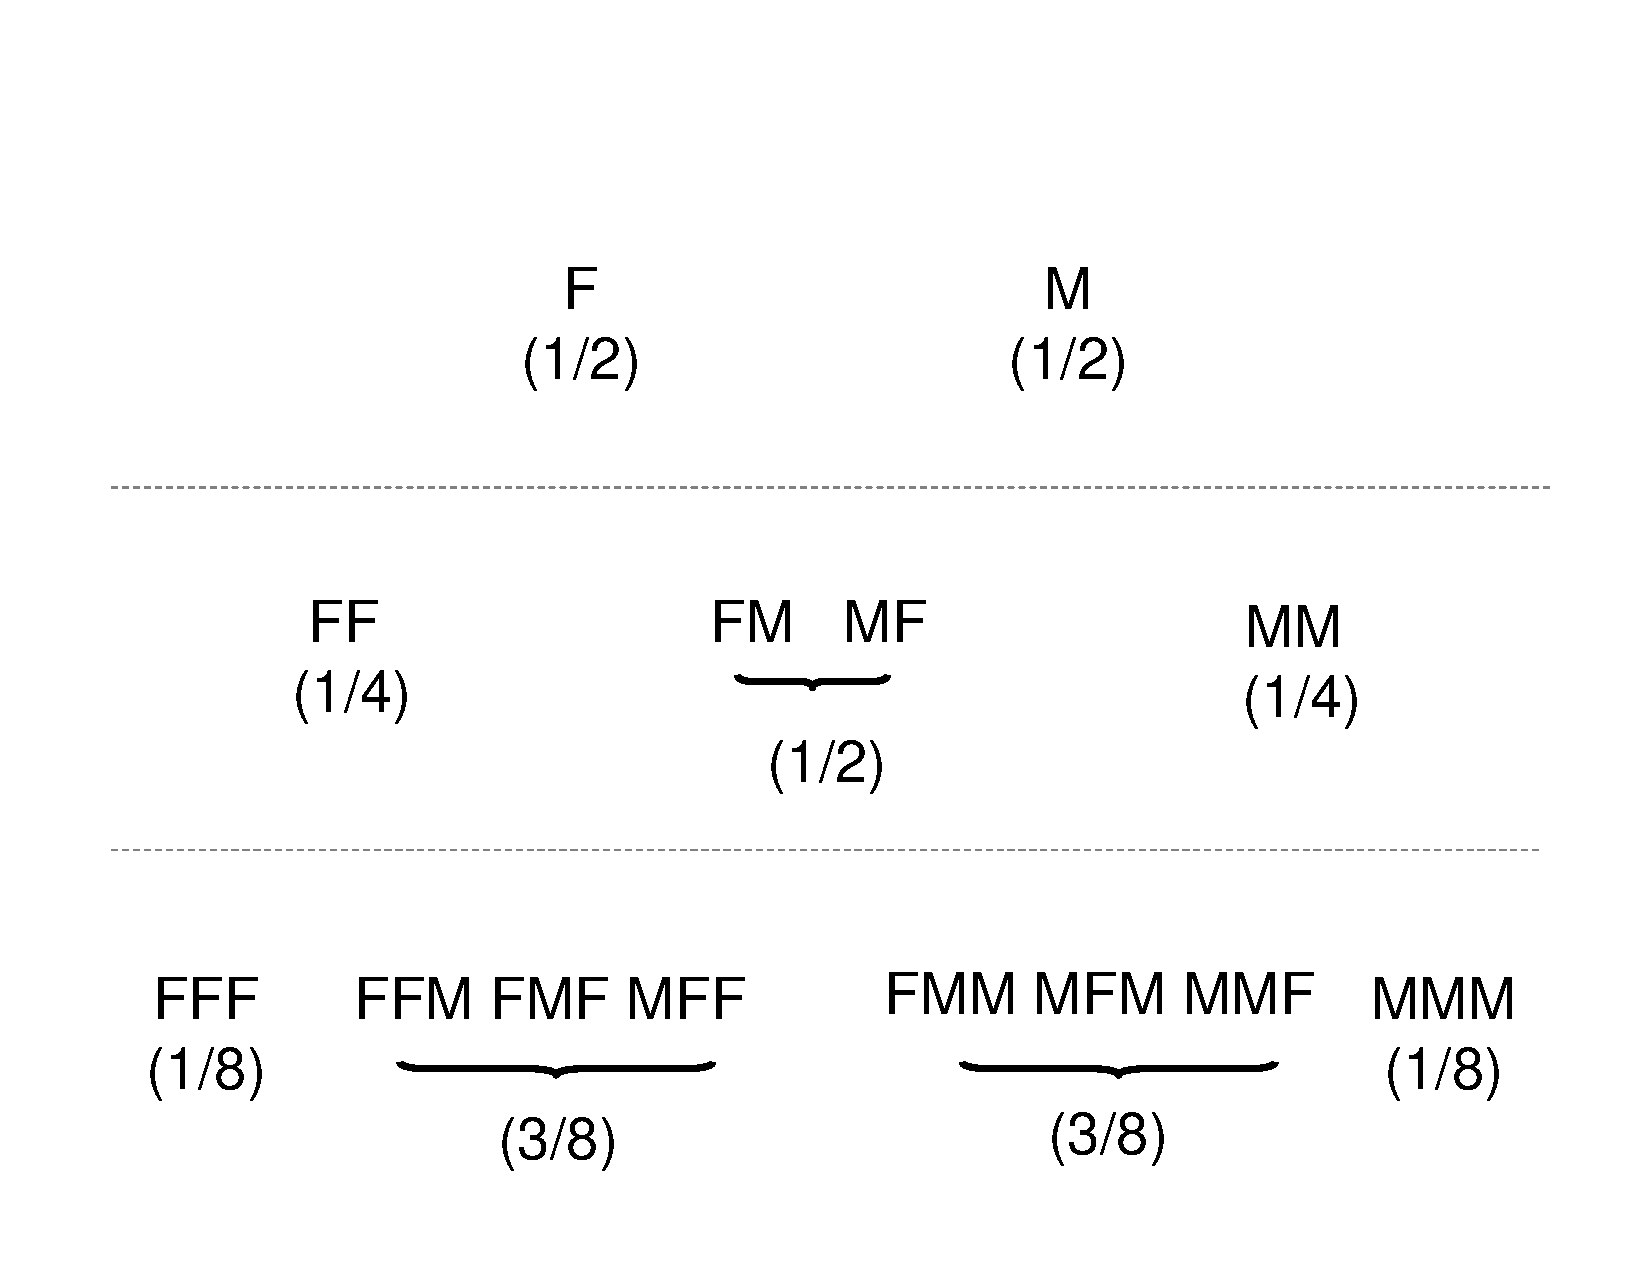
\includegraphics[scale=0.4,angle=270]{binomial.pdf}
		\end{center}
	\end{figure}
}



\frame{\frametitle{The binomial distribution} 
	
	Let $Y$ be the number of daughters a woman will have, $n$ the number of children
	she will have, and $p$ the probability of a daughter at any birth. Then: \\ \ \\
	\[ P(Y=k) =
	\frac{n!}{(n-k)!k!}p^k(1-p)^{(n-k)}\] \ \\ \ \\ where $n! =
	1\times2\times3\times ... \times (n-1)\times n$, and $0!=1$. \\ \ \\

	
	}

\begin{frame}[fragile]{Calculating binomial probabilities in R}
$P(Y=3) = \frac{3!}{0!3!}0.5^3(1-0.5)^{0}$ \\ \ \\
which can be solved in R using:
\begin{knitrout}\scriptsize
\definecolor{shadecolor}{rgb}{0.969, 0.969, 0.969}\color{fgcolor}
\begin{alltt}
\hlstd{stats}\hlopt{::}\hlkwd{dbinom}\hlstd{(}\hlkwc{x} \hlstd{=} \hlnum{3}\hlstd{,} \hlkwc{size} \hlstd{=} \hlnum{3}\hlstd{,} \hlkwc{prob} \hlstd{=} \hlnum{0.5}\hlstd{)}
\end{alltt}
\begin{verbatim}
## [1] 0.125
\end{verbatim}

\end{knitrout}
\end{frame}

\begin{frame}[fragile]{The probability mass function (pmf)}

\begin{knitrout}\scriptsize
\definecolor{shadecolor}{rgb}{0.969, 0.969, 0.969}\color{fgcolor}
\begin{alltt}
\hlkwd{plot}\hlstd{(}\hlnum{0}\hlopt{:}\hlnum{3}\hlopt{/}\hlnum{3}\hlstd{,} \hlkwd{dbinom}\hlstd{(}\hlkwc{x} \hlstd{=} \hlnum{0}\hlopt{:}\hlnum{3}\hlstd{,} \hlkwc{size} \hlstd{=} \hlnum{3}\hlstd{,} \hlkwc{prob} \hlstd{=} \hlnum{0.5}\hlstd{),} \hlkwc{type} \hlstd{=} \hlstr{"h"}\hlstd{)}
\end{alltt}


{\centering 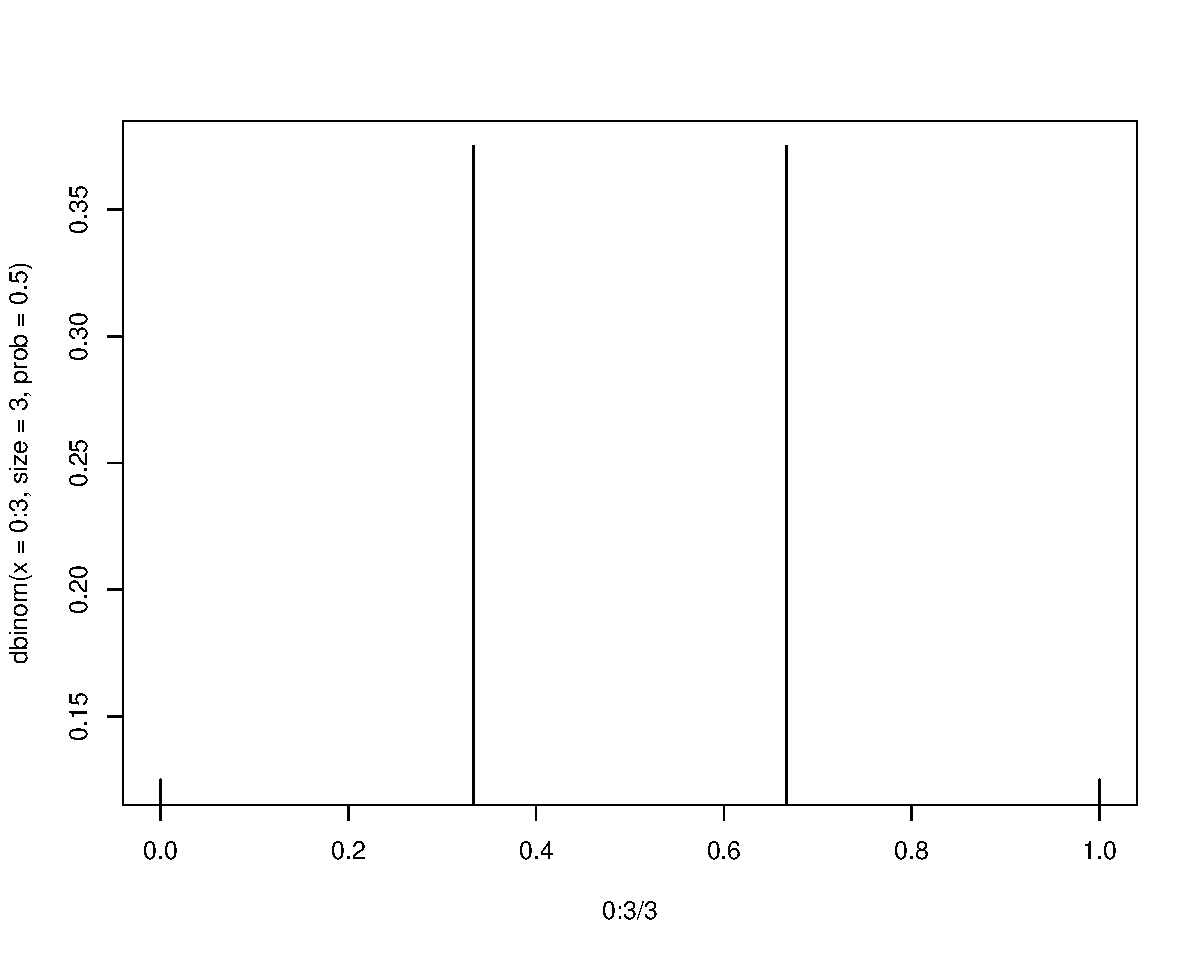
\includegraphics[width=1\linewidth]{figure/unnamed-chunk-2-1} 

}



\end{knitrout}
\end{frame}

\begin{frame}[fragile]{What do we use it for?}
\small
\begin{itemize}
	\setlength\itemsep{0.7em}
	\item to make inferences about $\pi$ from  observed  proportion $p= y/n.$ \pause 
	\item to make inferences in more complex situations, e.g. 
	\begin{itemize}
			\setlength\itemsep{0.4em}
		\item Prevalence Difference: $\pi _{1} - \pi _{0}$
		\item Risk Difference (RD): $\pi _{1} - \pi _{0}$
		\item Risk Ratio, or its synonym Relative Risk (RR): $\pi _{1}\:/\:\pi _{0}$
		\item Odds Ratio (OR): $[\: \pi _{1}/(1-\pi _{1})\:] \: / \: [\: \pi _{0}\: / \: (1-\pi _{0}) \: ]$
		\item Trend in several $\pi $'s
	\end{itemize}
\end{itemize}
\end{frame}


\frame{\frametitle{Requirements for $y$ to have a Binomial (n, $\pi $) distribution} 
	\begin{enumerate}
\item Fixed sample size $n.$ \pause
\item Elements selected at random (i.e. same probability of being sampled) and independent of each other;
\item Each element in ``population'' is 0 or 1, but we are only interested in estimating proportion  ($\pi $) of 1's;  we are not interested in individuals. \pause
\item Denote by $y_{i}$ the value of the $i$-th sampled element.  P($y_{i}=1)$ is constant (it is $\pi$) across $i$.
\end{enumerate} }


\begin{frame}
\begin{figure}
	\begin{center}
		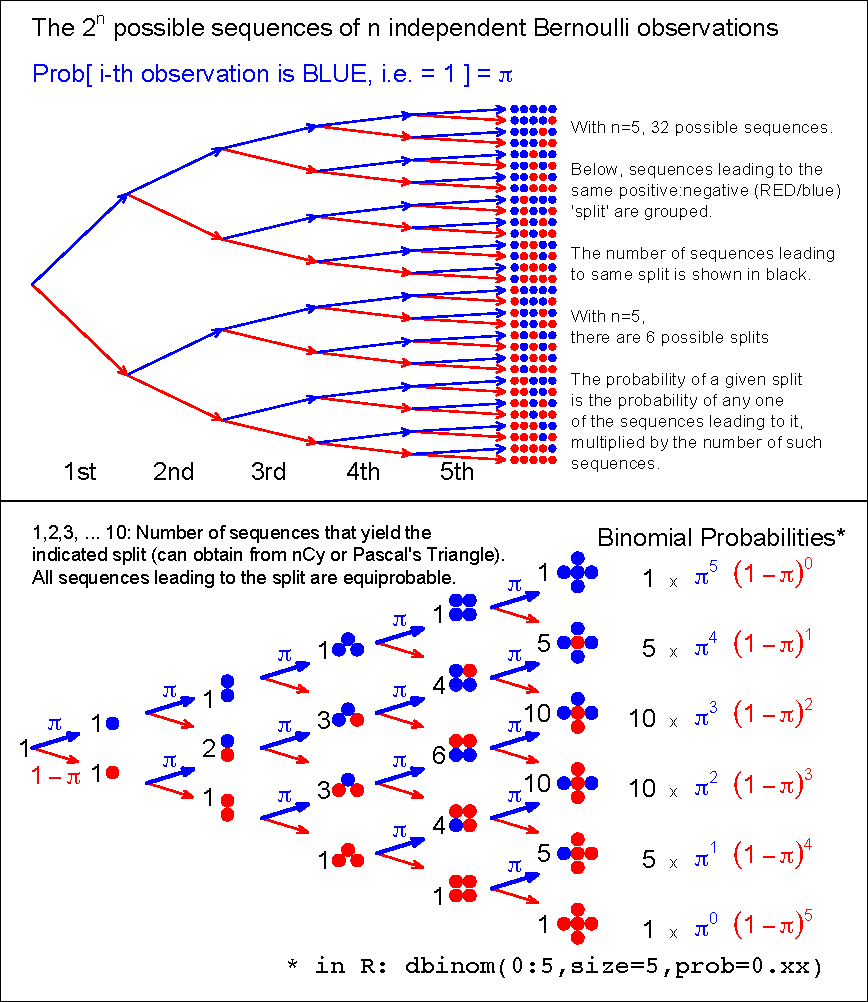
\includegraphics[scale=0.55]{BinomialTree2018.pdf}
		\caption{\scriptsize From 5 (independent and identically distributed) Bernoulli observations to Binomial $(n=5), \: \pi \textrm{ unspecified}$.}
			%There are $2^n$ possible (distinct) sequences of 0's and 1's, each with its probability. We are not interested in these $2^n$ probabilities, but in the probability that the sample  contains $y$ 1's and $(n-y)$ 0's. There are only ($n$+1) possibilities for $y$, namely 0 to $n.$ Fortunately, each of the $nC_y$ sequences that lead to the same sum or count ($y$), has the same probability. So we group the 2$^n$ sequences into $(n+1)$ sets, according to the sum or count. Each sequence in the set with  $y$ 1's and $(n-y)$ 0's has the same probability, namely $\pi ^{y}(1-\pi )^{n-y}$. Thus, in lieu of adding all such probabilities, we simply multiply this  probability by the number, $^{n}C _{y}$ -- shown in black -- of unique sequences in the set. Check: the numbers in black add to 2$^n.$ Nowadays, the $(n+1)$ probabilities are easily obtained by supplying a value for the \texttt{prob} argument in the \texttt{R} function \texttt{dbinom}, instead of  computing the binomial coefficient $nC_y$ by hand.}
	\end{center}
\end{figure}
\end{frame}


\begin{frame}{Does the Binomial Distribution Apply if... ?}

\small
\begin{tabular}{lrl}
	\hline
	Interested in & $\pi$      &  the proportion of 16 year old girls  \\
	&              &   in Qu\'{e}bec protected against rubella \\
	& & \\
	Choose        & $n=100$ & girls: 20 at random from each of 5 randomly \\
	&                &selected schools [`cluster' sample] \\
	& & \\
	Count & $y$ & how many of the $n=100$  are protected \\
	& & \\
	
	\multicolumn{3}{l}{$\bullet$ Is $y \sim \textrm{Binomial}(n = 100, \pi $)? } \\
	\hline
	& & \\
	``SMAC'' & $\pi$      &   P(abnormal$\:|\:$Healthy) =0.03 for each chemistry \\
	& &                       in Auto-analyzer with $n=18$ channels  \\
	&         &  \\
	Count            & y$ $&  How many of $n=18$  give abnormal result.  \\
	& & \\
	\multicolumn{3}{l}{$\bullet$ Is $y \sim \textrm{Binomial}(n = 18, \pi =0.03$)? (cf. Ingelfinger: Clin. Biostatistics) } 
\end{tabular}
\end{frame}


\begin{frame}{Does the Binomial Distribution Apply if... ?}

\small
\begin{tabular}{lrl}
	\hline
	
	Interested in & $\pi _{u}$      &   proportion in `usual' exercise classes and in  \\
	& $\pi _{e}$      &   expt'l. exercise classes who `stay the course'  \\
	& & \\
	Randomly & 4   & classes of\\ 
	Allocate    &  \underline{25} & students each to usual course \\
	& $n_{u} = 100$ &  \\
	& 4  & classes of\\
	&  \underline{25} & students each to experimental course \\
	& $n_{e} =100$ &  \\
	
	Count & $y_u$ & how many of the $n_{u}=100$ complete course \\
	& $y_e$ & how many of the $n_{e}=100$  complete course \\
	
	\multicolumn{3}{l}{$\bullet$ Is $y_{u} \sim \textrm{Binomial}(n_{u} = 100,  \pi _{u}$) ?
		\ \  Is $y_{e} \sim \textrm{Binomial}(n_{e} = 100,  \pi _{e}$) ?} \\
	& & \\
	\hline
\end{tabular}
\end{frame}



\begin{frame}{Does the Binomial Distribution Apply if... ?}

\small
\begin{tabular}{lrl}
	\hline
	Sex Ratio & $n=4$& children in each family  \\
	& $y$ & number of girls in family \\
	& & \\
	\multicolumn{3}{l}{$\bullet$ Is variation of y across families Binomial (n = 4, $\pi $ = 0.49)?} \\
	\hline
	Pilot  &   &To estimate proportion $\pi$ of population that\\ 
	Study&   &  is eligible \& willing to participate in long-term\\
	&   & research study, keep recruiting until obtain   \\
	& $y=5$ &  who are. Have to approach $n$ to get $y$. \\
	& & \\
	\multicolumn{3}{l}{$\bullet$ Can we treat $y \sim \textrm{Binomial}(n, \pi$)?} \\
	\hline
\end{tabular}
\end{frame}


\begin{frame}{Calculating Binomial probabilities - Exactly}



\begin{itemize}
	\item  probability mass function (pmf): $P(Y=k) =
	\frac{n!}{(n-k)!k!}p^k(1-p)^{(n-k)}$
	\item in \texttt{R}: \texttt{dbinom(), pbinom(), qbinom()}: \newline probability mass, distribution/cdf, and quantile functions.
\end{itemize}

\end{frame}




\begin{frame}{Calculating Binomial probabilities - Using an approximation}

\small
\begin{itemize}
	\item Poisson Distribution ($n$ large;  small $\pi$)
	\item Normal (Gaussian) Distribution ($n$ large or midrange $\pi $) \footnote{\footnotesize
		For when you don't have access to software or Tables, e.g, on a plane} 
	\begin{itemize}
		\item Have to specify \textit{scale}. Say $n=10$, whether summary is a 
		\begin{tabular}{rllcc}
			&  \textbf{r.v. }        &  \textbf{e.g.} & \textbf{E} & \textbf{SD} \\ 
			\hline
			count:          &  $y$        &  2 & $n \times \pi$ & $\{n \times \pi \times (1-\pi) \}^{1/2}$ \\
			& & & & \\
			& & & & $n^{1/2} \times \sigma_{Bernoulli}$ \\
			
			& & & & \\
			proportion:   & $p=y/n$  & 0.2 & $ \pi$ & $\{\pi \times (1-\pi) / n \}^{1/2}$ \\
			& & & & \\
			
			& & & &  $\sigma_{Bernoulli} / n^{1/2}$\\
			
			& & & & \\
			percentage: &$100p\%$ & 20\% & $100 \times \pi$ & $100 \times SD[p]$ \\
			\hline
		\end{tabular}
		\item same core calculation for all 3 [only the \textit{scale} changes]. JH prefers (0,1), the same scale as $\pi.$
		
	\end{itemize}
	
\end{itemize}

\end{frame}



\begin{frame}[fragile]{Normal approximation to binomial is the CLT in action}
\begin{knitrout}\scriptsize
\definecolor{shadecolor}{rgb}{0.969, 0.969, 0.969}\color{fgcolor}

{\centering 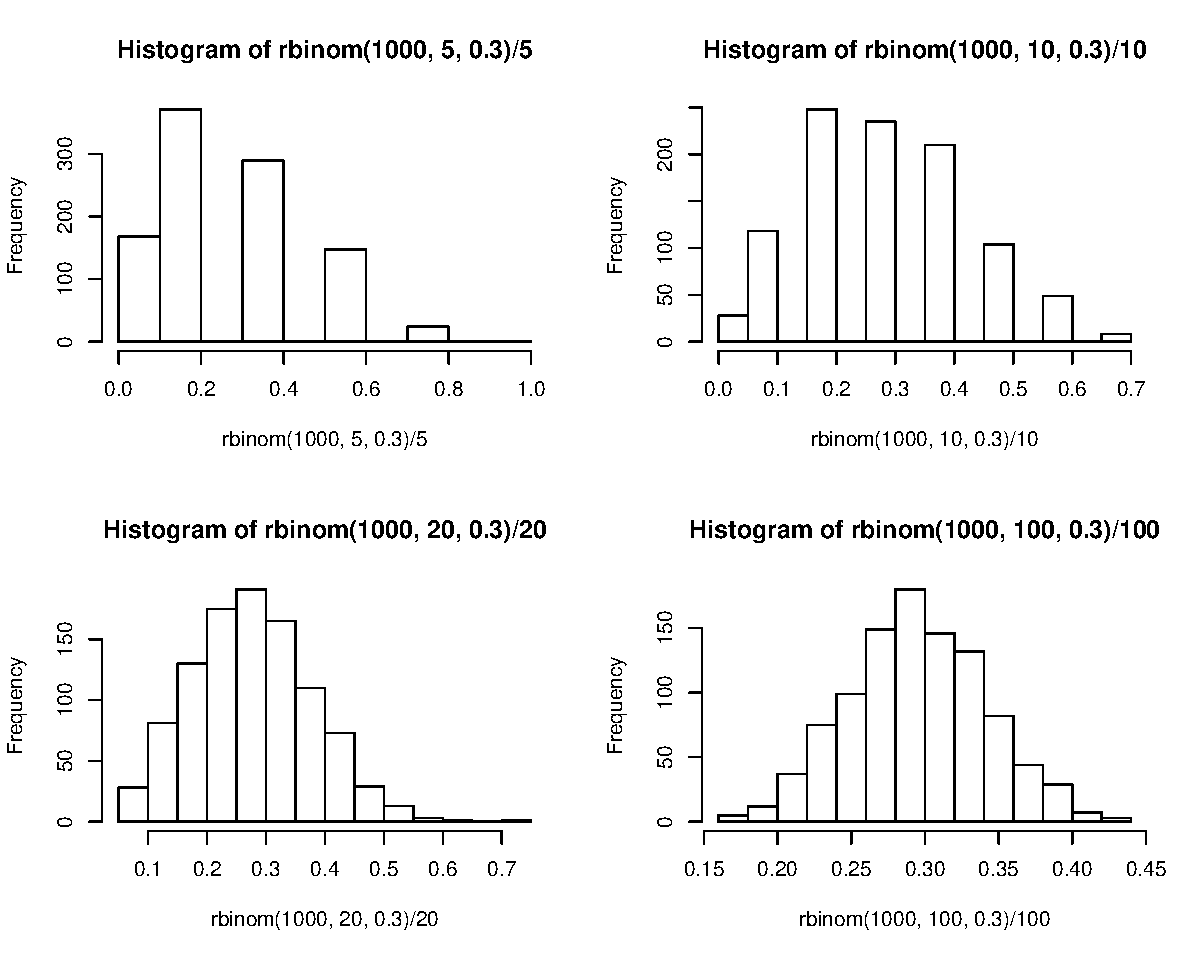
\includegraphics[width=1\linewidth]{figure/unnamed-chunk-3-1} 

}



\end{knitrout}
\end{frame}


\begin{frame}[fragile]{Normal approximation to binomial is the CLT in action}
\begin{knitrout}\scriptsize
\definecolor{shadecolor}{rgb}{0.969, 0.969, 0.969}\color{fgcolor}

{\centering 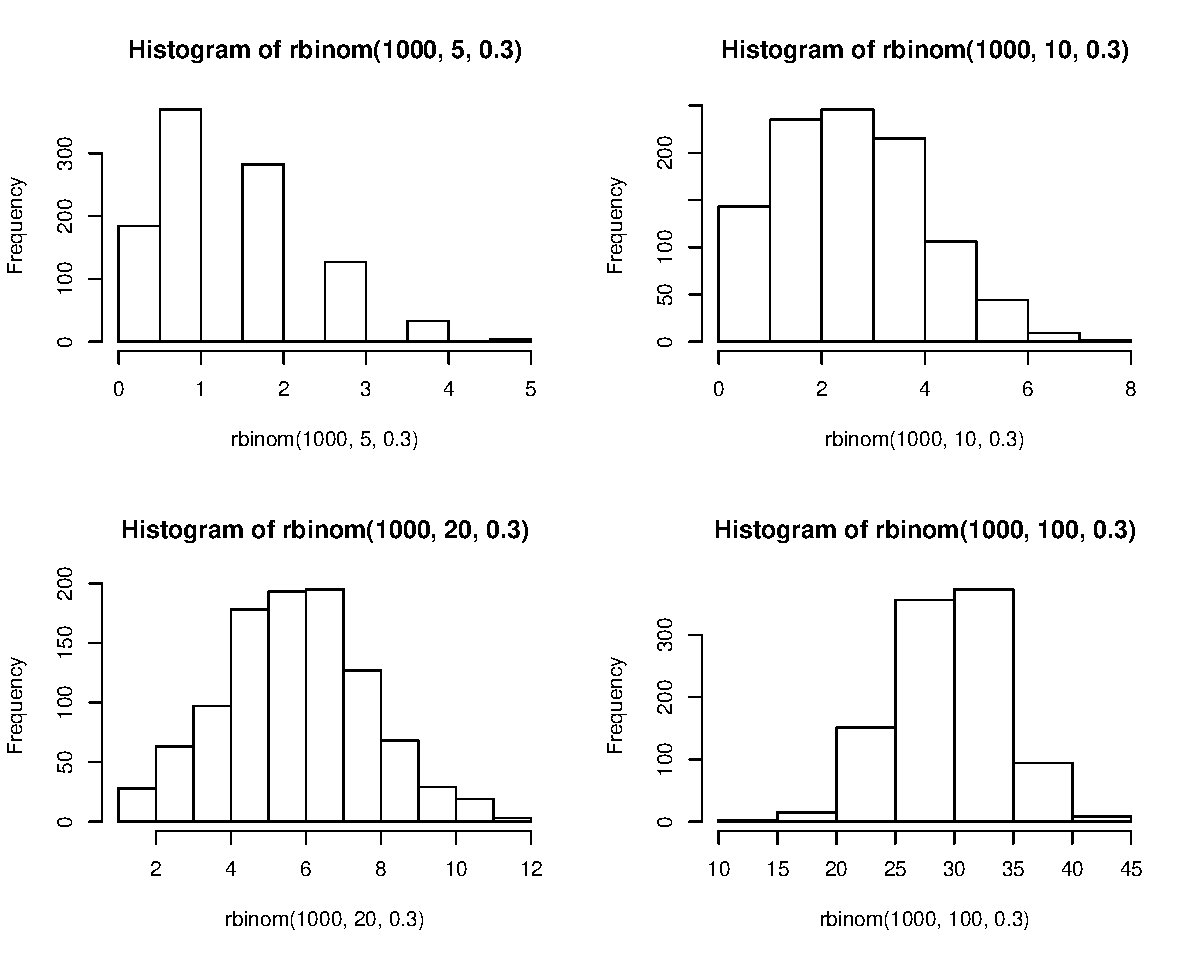
\includegraphics[width=1\linewidth]{figure/unnamed-chunk-4-1} 

}



\end{knitrout}
\end{frame}

\begin{frame}{Example from AAO Unit 21}
A drug manufacturer claims that its flu vaccine is 85\% effective; in other words, each person who is vaccinated stands an 85\% chance of developing immunity. Suppose that 200 randomly selected people are vaccinated. Let $Y$ be the number that develops immunity.

\begin{enumerate}
	\item What is the distribution of $Y$?
\item What is the mean and standard deviation for $Y$?
\item What is the probability that between 165 and 180 of the 200 people who were vaccinated
develop immunity? (Hint: Use a normal distribution to approximate the distribution of $Y$)
\end{enumerate}
\end{frame}


\begin{frame}[fragile]{Example from AAO Unit 21 - Exact Method}

\begin{knitrout}\scriptsize
\definecolor{shadecolor}{rgb}{0.969, 0.969, 0.969}\color{fgcolor}
\begin{alltt}
\hlstd{mosaic}\hlopt{::}\hlkwd{xpbinom}\hlstd{(}\hlkwc{q} \hlstd{=} \hlkwd{c}\hlstd{(}\hlnum{165}\hlstd{,} \hlnum{180}\hlstd{),} \hlkwc{size} \hlstd{=} \hlnum{200}\hlstd{,} \hlkwc{prob} \hlstd{=} \hlnum{0.85}\hlstd{)}
\end{alltt}


{\centering 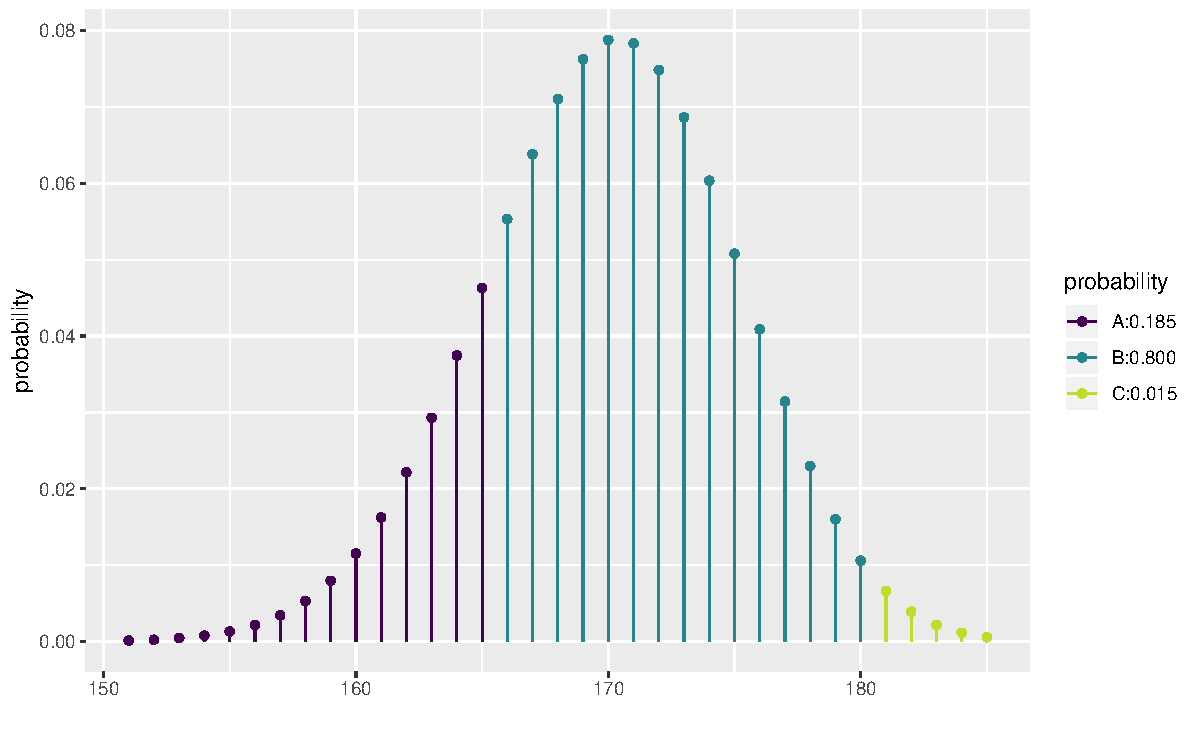
\includegraphics[width=1\linewidth]{figure/unnamed-chunk-5-1} 

}


\begin{verbatim}
## [1] 0.1850410 0.9851197
\end{verbatim}

\end{knitrout}
\end{frame}

\begin{frame}[fragile]{Example from AAO Unit 21- Normal Approximation}

\begin{knitrout}\scriptsize
\definecolor{shadecolor}{rgb}{0.969, 0.969, 0.969}\color{fgcolor}
\begin{alltt}
\hlstd{mosaic}\hlopt{::}\hlkwd{xpnorm}\hlstd{(}\hlkwc{q} \hlstd{=} \hlkwd{c}\hlstd{(}\hlnum{165}\hlstd{,}\hlnum{180}\hlstd{),} \hlkwc{mean} \hlstd{=} \hlnum{200} \hlopt{*} \hlnum{0.85}\hlstd{,}
        \hlkwc{sd} \hlstd{=} \hlkwd{sqrt}\hlstd{(}\hlnum{200}\hlopt{*}\hlnum{0.85}\hlopt{*}\hlnum{0.15}\hlstd{))}
\end{alltt}


{\centering 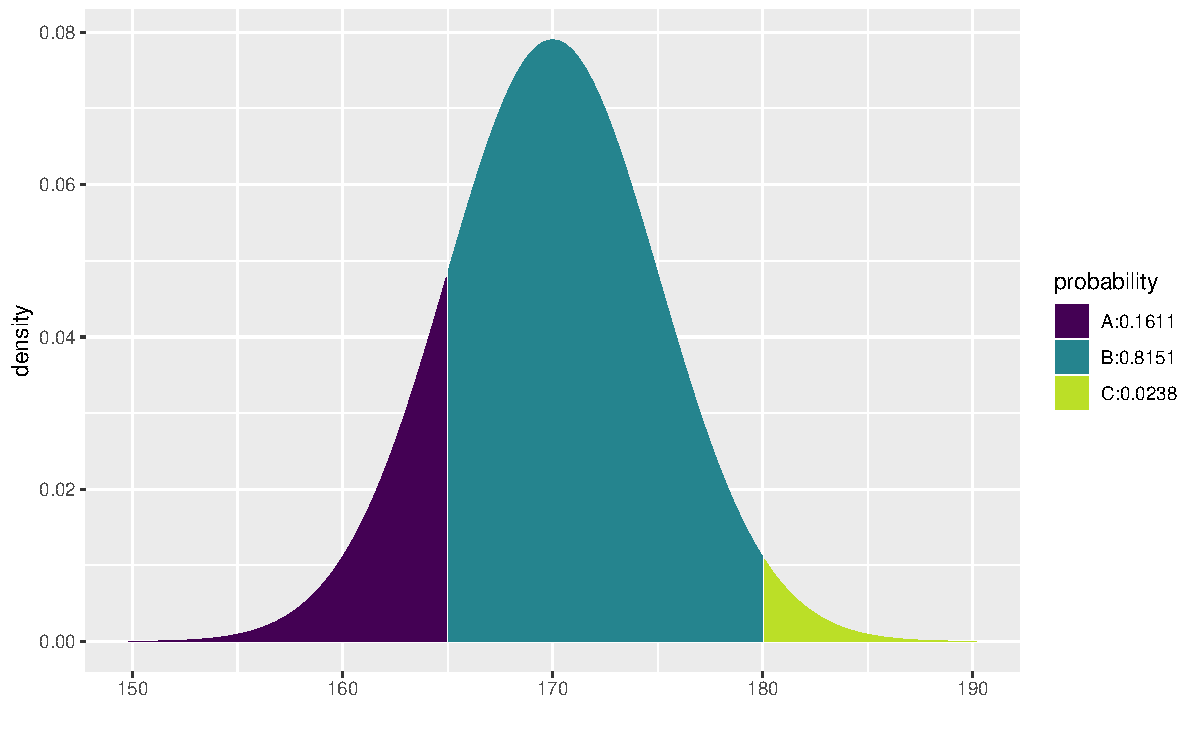
\includegraphics[width=1\linewidth]{figure/unnamed-chunk-6-1} 

}


\begin{verbatim}
## [1] 0.1610510 0.9761648
\end{verbatim}

\end{knitrout}
\end{frame}


\end{document}











